\pagestyle{empty}

% Set PATH
\renewcommand{\PATH}{../..}

% Row i II
\newcommand{\rowiIIheight}{.11\textheight}
\newcommand{\rowiIIhjust}{.75}
\newcommand{\rowiIIvjust}{.5}

% Figure S1
\renewcommand{\figurename}{Supplementary Figure}
\setcounter{figure}{0}

\begin{figure}
	\begin{tikzpicture}
		\node[anchor=north west] at (0,0) {
			\includegraphics[width=\textwidth]{\PATH/analysis/BCB/overview/sample-overview.png}};
		\node[anchor=north east] at (1,1) {\textbf{\LARGE{A}}};
	\end{tikzpicture}
	\begin{tikzpicture}
		\node[anchor=north west] at (0,0) {
			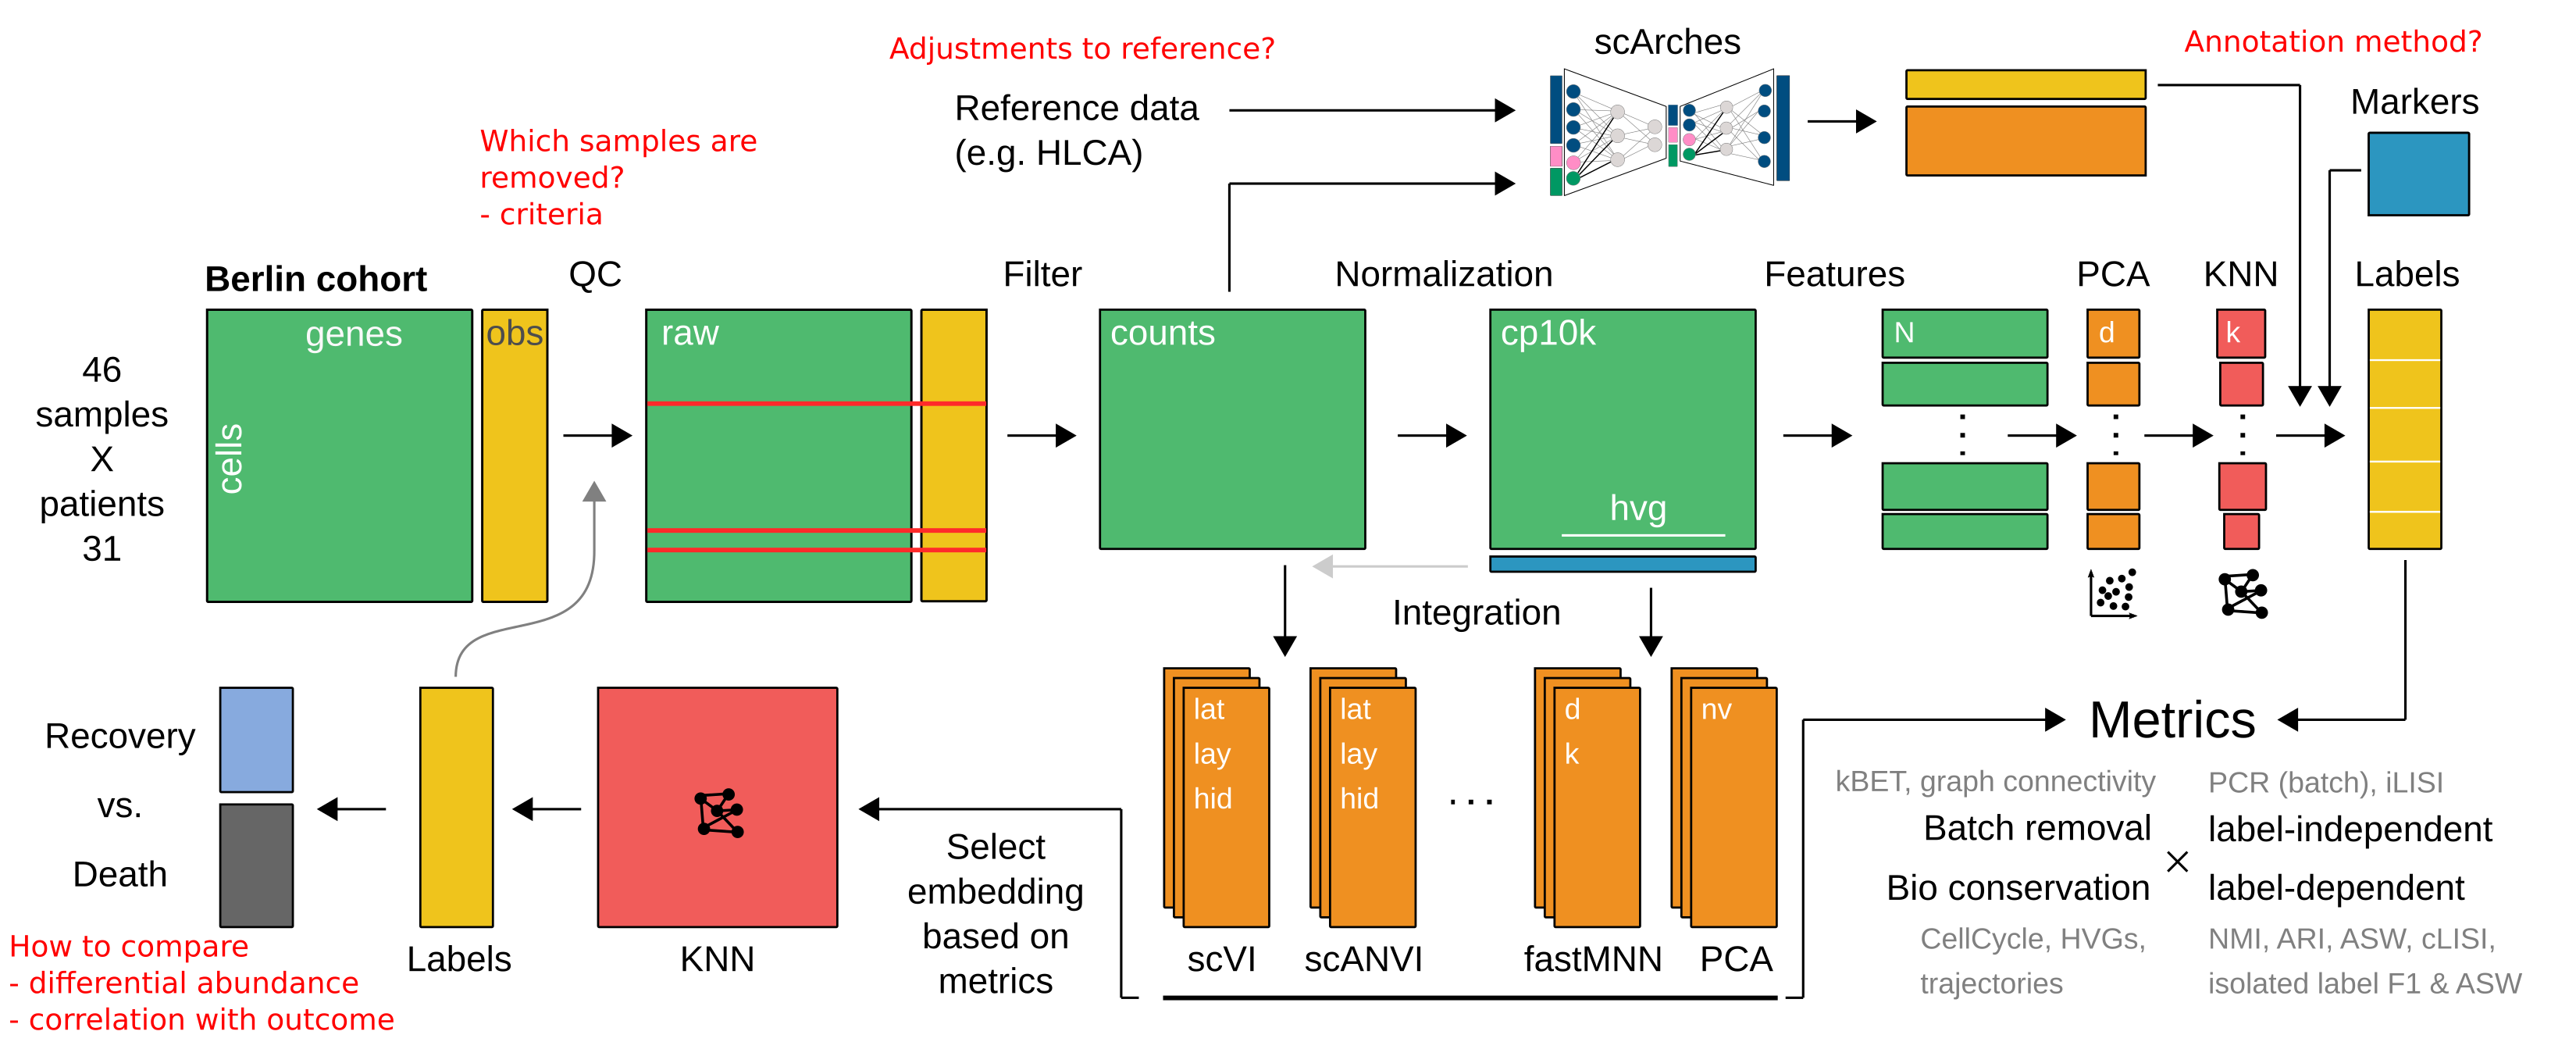
\includegraphics[width=\textwidth]{\PATH/docs/workflow/main.png}};
		\node[anchor=north east] at (1,0) {\textbf{\LARGE{B}}};
	\end{tikzpicture}
	
	\caption{Cell type diversity in bronchoalveolar lavage (BAL) fluid in severe COVID-19. A) Overview of the samples included in the dataset of BALs from severe COVID-19. B) Computational workflow for the analysis of BAL samples focused on the selection of the best integration method. Further, per-sample quality control and automated cell annotation are major goals. In the end, comparison of cellular composition across disease outcomes should lead to new insights.}
\end{figure}